\documentclass[11pt]{beamer}
\usetheme{Madrid}
\usepackage[utf8]{inputenc}
\usepackage{amsmath}
\usepackage{amsfonts}
\usepackage{amssymb}
\usepackage{graphicx}
\usepackage{xcolor}
\usepackage{tikz}
\usepackage{geometry}
\usepackage{array}
\usepackage{longtable}

\title{EB1A \& EB2-NIW Post-Denial Strategy}
\subtitle{Master-Class Post-Adjudication Framework \& Strategic Litigation Tactics}
\author{Advanced Post-Adjudication Training System}
\date{\today}

\setbeamercovered{transparent}
\setbeamertemplate{navigation symbols}{}
\setbeamerfont{itemize/enumerate body}{size=\scriptsize}
\setbeamerfont{itemize/enumerate subbody}{size=\tiny}
\setbeamerfont{block body}{size=\scriptsize}
\setbeamerfont{block title}{size=\normalsize}

\begin{document}
	
	% ============================================================
	% TITLE SLIDE
	% ============================================================
	\begin{frame}
		\titlepage
		\centering
		\scriptsize \textit{What to Do After a USCIS Denial: The Complete Post-Denial Workflow}
	\end{frame}
	
	% ============================================================
	% SECTION 1: THE COMPLETE WORKFLOW MAP (NEW - 10 SLIDES)
	% ============================================================
	
	\begin{frame}{The Complete Post-Denial Workflow: 6-Step Sequence}
		\scriptsize
		\begin{block}{The Master Sequence You Will Learn}
			\textbf{Step 1:} Receive USCIS Denial
			\vspace{0.1cm}
			\textbf{Step 2:} File Motion to Reopen (MTR) within 30 days
			\vspace{0.1cm}
			\textbf{Step 3:} If USCIS delays MTR decision beyond 6 months → File Mandamus to force decision
			\vspace{0.1cm}
			\textbf{Step 4:} After USCIS denies MTR → File Motion to Reconsider (MTC) within 30 days
			\vspace{0.1cm}
			\textbf{Step 5:} After MTC denied → Send Pre-Litigation Notice (30-60 day warning)
			\vspace{0.1cm}
			\textbf{Step 6:} File APA Complaint in Federal District Court
		\end{block}
	\end{frame}
	
	\begin{frame}{The Complete Post-Denial Workflow: Visual Map}
		\scriptsize
		\begin{center}
			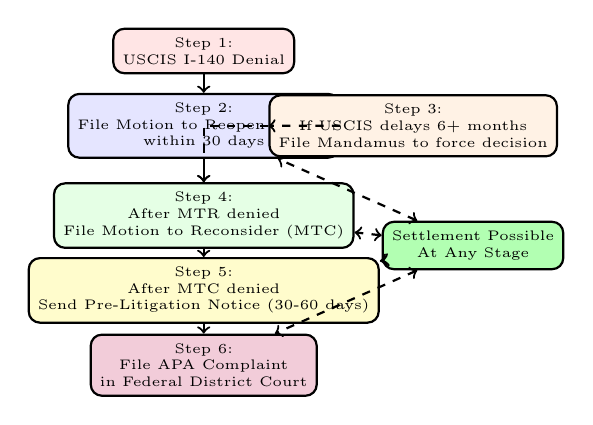
\begin{tikzpicture}[scale=0.38, every node/.style={draw, rounded corners, align=center, font=\tiny}]
				\node (denial) at (0,0) [fill=red!10, draw=black, thick] {Step 1:\\USCIS I-140 Denial};
				\node (mtr) at (0,-2.5) [fill=blue!10, draw=black, thick] {Step 2:\\File Motion to Reopen (MTR)\\within 30 days};
				\node (mandamus) at (7,-2.5) [fill=orange!10, draw=black, thick] {Step 3:\\If USCIS delays 6+ months\\File Mandamus to force decision};
				\node (mtc) at (0,-5.5) [fill=green!10, draw=black, thick] {Step 4:\\After MTR denied\\File Motion to Reconsider (MTC)};
				\node (notice) at (0,-8) [fill=yellow!20, draw=black, thick] {Step 5:\\After MTC denied\\Send Pre-Litigation Notice (30-60 days)};
				\node (apa) at (0,-10.5) [fill=purple!20, draw=black, thick] {Step 6:\\File APA Complaint\\in Federal District Court};
				\node (settle) at (9,-6.5) [fill=green!30, draw=black, thick] {Settlement Possible\\At Any Stage};
				
				\draw[->, thick] (denial) -- (mtr);
				\draw[->, thick] (mtr) -- (mtc);
				\draw[->, thick] (mtc) -- (notice);
				\draw[->, thick] (notice) -- (apa);
				\draw[->, dashed, thick] (mtr) -- (mandamus);
				\draw[->, dashed, thick] (mandamus) -| (mtc);
				\draw[<->, dashed, thick] (settle) -- (mtr);
				\draw[<->, dashed, thick] (settle) -- (mtc);
				\draw[<->, dashed, thick] (settle) -- (notice);
				\draw[<->, dashed, thick] (settle) -- (apa);
			\end{tikzpicture}
		\end{center}
	\end{frame}
	
	\begin{frame}{The "Commitment Mistake" in MTR Explained}
		\scriptsize
		\begin{block}{What Is the "Commitment Mistake"?}
			Many applicants file a Motion to Reopen without understanding a critical requirement:
			\vspace{0.2cm}
			\textcolor{red}{\textbf{You cannot file an MTR just because you disagree with the decision.}}
			\vspace{0.2cm}
			\textbf{The MTR Standard (8 C.F.R. § 103.5(a)(2)):}
			\begin{itemize}
				\item You must present \textbf{new, material facts}
				\item That were \textbf{not available and could not have been discovered} at the time of the original filing
				\item Supported by \textbf{affidavits or documentary evidence}
			\end{itemize}
			\textcolor{blue}{The "commitment mistake" is filing an MTR based only on legal disagreement, not on new facts.}
		\end{block}
	\end{frame}
	
	\begin{frame}{Commitment Mistake: Legal Disagreement vs. New Facts}
		\scriptsize
		\begin{block}{What USCIS Will Reject (Commitment Mistake)}
			\begin{quote}
				``I disagree with the officer's conclusion that my endeavor lacks national importance. The officer should have found that my work qualifies.''
			\end{quote}
			\textbf{Why this fails:} This is a legal disagreement, not a new fact. The officer already considered your evidence and disagreed.
			\vspace{0.3cm}
			\textbf{What USCIS Will Accept (Proper MTR):}
			\begin{quote}
				``New expert declaration (Exhibit A) from Dr. Smith, who was not available at the time of filing, confirms that my quantitative methodology was fully operational prior to the filing date. This new evidence directly addresses the officer's finding that the endeavor lacked operational capability.''
			\end{quote}
			\textcolor{green}{This is a new, material fact that existed but could not be presented earlier.}
		\end{block}
	\end{frame}
	
	\begin{frame}{Why Mandamus Is Needed After MTR Filing}
		\scriptsize
		\begin{block}{The Mandamus Step: When USCIS Won't Decide}
			After you file a Motion to Reopen (MTR), USCIS may:
			\vspace{0.2cm}
			\begin{itemize}
				\item Sit on your motion for 6, 9, 12+ months
				\item Ignore your status inquiries
				\item Leave you in administrative limbo
			\end{itemize}
			\textbf{Without Mandamus:}
			\begin{itemize}
				\item You cannot move to the next step (MTC or federal court)
				\item Your case is stuck indefinitely
				\item USCIS has no legal obligation to decide quickly (no statutory deadline)
			\end{itemize}
			\textcolor{red}{Mandamus is the tool to force USCIS to issue a decision on your pending MTR.}
		\end{block}
	\end{frame}
	
	\begin{frame}{Mandamus Timeline: When to File}
		\scriptsize
		\begin{block}{Strategic Timing for Mandamus After MTR}
			\begin{tabular}{|p{3cm}|p{6cm}|}
				\hline
				\textbf{Time Since MTR Filing} & \textbf{Recommended Action} \\
				\hline
				0-3 months & Normal processing; wait \\
				\hline
				3-4 months & Send first status inquiry via phone/email \\
				\hline
				4-5 months & Send second status inquiry (written) \\
				\hline
				5-6 months & Send formal pre-mandamus notice to USCIS \\
				\hline
				6-8 months & File Mandamus complaint in federal court \\
				\hline
				8-12 months & Strong mandamus case (delay clearly unreasonable) \\
				\hline
				12+ months & Very strong mandamus case; likely to succeed \\
				\hline
			\end{tabular}
		\end{block}
	\end{frame}
	
	\begin{frame}{MTC: Challenge Both Denials}
		\scriptsize
		\begin{block}{Bundled Legal Challenges in MTC}
			Your Motion to Reconsider should challenge:
			\vspace{0.2cm}
			\textbf{Original I-140 Denial Errors:}
			\begin{itemize}
				\item Heightened standard error (field domination requirement)
				\item Evidentiary fragmentation
				\item Ignored expert opinion letters
				\item Prospective vs. realized impact confusion
			\end{itemize}
			\textbf{MTR Denial Errors:}
			\begin{itemize}
				\item Misapplication of \textit{Matter of Katigbak}
				\item Failure to recognize clarifying evidence as permissible
				\item Categorically rejecting new expert letters
				\item Arbitrary dismissal of pre-filing documentation
			\end{itemize}
			\textcolor{red}{A single MTC can (and should) challenge both denials simultaneously.}
		\end{block}
	\end{frame}
	
	\begin{frame}{Pre-Litigation Notice: What It Is}
		\scriptsize
		\begin{block}{Definition and Purpose}
			A Pre-Litigation Notice is a formal written communication sent to the government before filing a lawsuit.
			\vspace{0.2cm}
			\textbf{Purpose:}
			\begin{itemize}
				\item Notifies the government of your intent to sue
				\item Summarizes the legal errors in the agency's decisions
				\item Requests that the agency cure the errors within a specified timeframe
				\item Creates a record of good-faith effort to resolve without litigation
				\item Required by some courts before filing pro se
			\end{itemize}
			\textbf{Sent to:}
			\begin{itemize}
				\item DHS Secretary
				\item USCIS Director
				\item Service Center Director
				\item U.S. Attorney for your district
				\item Attorney General of the United States
			\end{itemize}
		\end{block}
	\end{frame}
	
	\begin{frame}{The Complete Post-Denial Flowchart (Full)}
		\scriptsize
		\begin{center}
			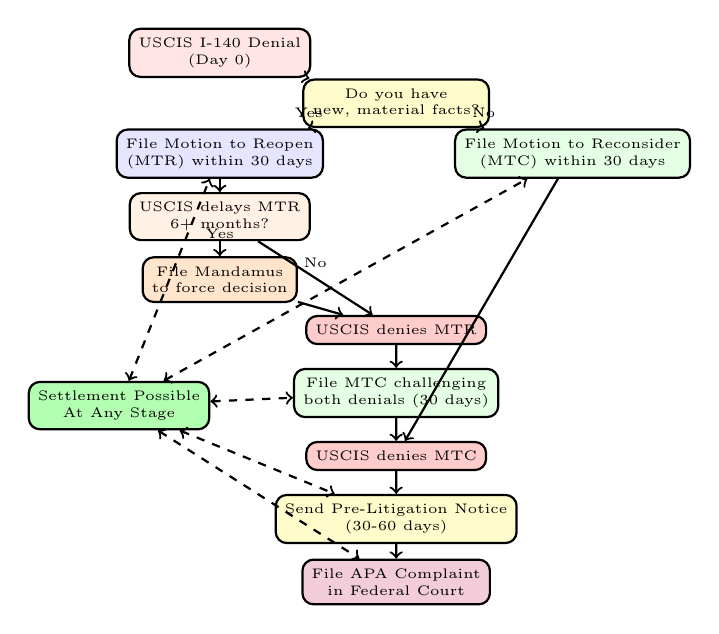
\begin{tikzpicture}[scale=0.32, every node/.style={draw, rounded corners, align=center, font=\tiny}]
				\node (denial) at (0,0) [fill=red!10, draw=black, thick] {USCIS I-140 Denial\\(Day 0)};
				\node (decision1) at (7,-2) [fill=yellow!20, draw=black, thick] {Do you have\\new, material facts?};
				\node (mtr) at (0,-4) [fill=blue!10, draw=black, thick] {File Motion to Reopen\\(MTR) within 30 days};
				\node (mtc) at (14,-4) [fill=green!10, draw=black, thick] {File Motion to Reconsider\\(MTC) within 30 days};
				\node (delay) at (0,-6.5) [fill=orange!10, draw=black, thick] {USCIS delays MTR\\6+ months?};
				\node (mandamus) at (0,-9) [fill=orange!20, draw=black, thick] {File Mandamus\\to force decision};
				\node (mtrdenied) at (7,-11) [fill=red!20, draw=black, thick] {USCIS denies MTR};
				\node (mtcfiling) at (7,-13.5) [fill=green!10, draw=black, thick] {File MTC challenging\\both denials (30 days)};
				\node (mtcdenied) at (7,-16) [fill=red!20, draw=black, thick] {USCIS denies MTC};
				\node (notice) at (7,-18.5) [fill=yellow!20, draw=black, thick] {Send Pre-Litigation Notice\\(30-60 days)};
				\node (apa) at (7,-21) [fill=purple!20, draw=black, thick] {File APA Complaint\\in Federal Court};
				\node (settle) at (-4,-14) [fill=green!30, draw=black, thick] {Settlement Possible\\At Any Stage};
				
				\draw[->, thick] (denial) -- (decision1);
				\draw[->, thick] (decision1) -- node[above, draw=none] {Yes} (mtr);
				\draw[->, thick] (decision1) -- node[above, draw=none] {No} (mtc);
				\draw[->, thick] (mtr) -- (delay);
				\draw[->, thick] (delay) -- node[above, draw=none] {Yes} (mandamus);
				\draw[->, thick] (mandamus) -- (mtrdenied);
				\draw[->, thick] (delay) -- node[above, draw=none] {No} (mtrdenied);
				\draw[->, thick] (mtrdenied) -- (mtcfiling);
				\draw[->, thick] (mtc) -- (mtcdenied);
				\draw[->, thick] (mtcfiling) -- (mtcdenied);
				\draw[->, thick] (mtcdenied) -- (notice);
				\draw[->, thick] (notice) -- (apa);
				\draw[<->, dashed, thick] (settle) -- (mtr);
				\draw[<->, dashed, thick] (settle) -- (mtc);
				\draw[<->, dashed, thick] (settle) -- (mtcfiling);
				\draw[<->, dashed, thick] (settle) -- (notice);
				\draw[<->, dashed, thick] (settle) -- (apa);
			\end{tikzpicture}
		\end{center}
	\end{frame}
	
	% ============================================================
	% SECTION 2: COURSE OVERVIEW & COMPLIANCE BOUNDARIES (ORIGINAL)
	% ============================================================
	
	\begin{frame}{What This Course Is (And Is Not)}
		\scriptsize
		\begin{block}{Course Purpose}
			\textbf{This course is NOT designed to promise that a denial will be overturned.}
			\vspace{0.1cm}
			\textbf{Instead, this course teaches:}
			\begin{itemize}
				\item Understanding the downstream impact of denials and their systemic consequences.
				\item Advanced strategies to mitigate structural timeline harm and protect your immigrant intent profile.
				\item Navigating post-denial remediation options, regulatory timelines, and jurisdictional safeguards.
				\item Executing precise litigation pressure to force favorable local actions outside of an appellate vacuum.
			\end{itemize}
			\textcolor{red}{\textbf{Legal Disclaimer:}} The instructor is not a licensed attorney, and this material does not constitute explicit legal advice. This is an informational framework mapping out procedural mechanics under 8 C.F.R. and 5 U.S.C.
		\end{block}
	\end{frame}
	
	% ============================================================
	% SECTION 3: UNDERSTANDING DENIAL PSYCHOLOGY (ORIGINAL)
	% ============================================================
	
	\begin{frame}{The Psychology Behind a USCIS Denial}
		\scriptsize
		\begin{block}{Why Officers Deny When They Could Approve}
			\textbf{Understanding the adjudicator's mindset is critical to crafting an effective response:}
			\vspace{0.1cm}
			\begin{itemize}
				\item \textbf{Cover Your Tracks Culture:} Officers face internal audits. Denying a borderline case creates less professional risk than approving one that later gets flagged.
				\item \textbf{Template-Driven Denials:} Many denials use boilerplate language from previous cases. The officer may have applied a standard template without deeply analyzing your specific evidence.
				\item \textbf{Lack of Subject Matter Expertise:} Officers are generalists. They may not understand technical fields like quantitative finance, AI architecture, or specialized engineering.
				\item \textbf{Time Pressure:} Officers handle hundreds of files. They may spend 15-30 minutes on a petition that represents years of your work.
			\end{itemize}
			\textcolor{blue}{Understanding this psychology helps you write briefs that overcome their natural hesitation.}
		\end{block}
	\end{frame}
	
	\begin{frame}{The Difference Between Legal Error and Factual Disagreement}
		\scriptsize
		\begin{block}{Two Types of Denial Problems}
			\textbf{Legal Error (Winnable via MTO/APA):}
			\begin{itemize}
				\item Officer applied the wrong legal standard (e.g., required "field domination" for NIW)
				\item Officer ignored binding precedent (\textit{Dhanasar}, \textit{Chawathe})
				\item Officer considered factors forbidden by regulation
				\item Officer failed to provide reasoned explanation for rejecting evidence
			\end{itemize}
			\textbf{Factual Disagreement (Harder to Win):}
			\begin{itemize}
				\item Officer simply disagrees with your interpretation of the evidence
				\item Officer believes your evidence is insufficient (weight, not type)
				\item Officer questions your credibility or the credibility of your experts
			\end{itemize}
			\textcolor{red}{Legal errors are much easier to overturn than factual disagreements.}
		\end{block}
	\end{frame}
	
	\begin{frame}{Why Denials Are "Sticky" and Dangerous}
		\scriptsize
		\begin{block}{Collateral Consequences of a Denial}
			\textbf{1. Credibility Perception and History Tracking:}
			\begin{itemize}
				\item USCIS officers consistently retrieve historical petition patterns from internal databases before evaluating a new filing.
				\item A standing denial establishes an adverse baseline record, increasing psychological barriers for subsequent adjudicators.
			\end{itemize}
			\textbf{2. Parallel Filings / Future Category Adjustments:}
			\begin{itemize}
				\item Moving from an EB-2 NIW profile to an EB-1A profile post-denial signals an inconsistent evidentiary pivot to the center.
				\item Adjudicators scrutinize the sudden escalation from "national importance" to "extraordinary ability."
			\end{itemize}
			\textbf{3. Permanent Disclosure Mandates:}
			\begin{itemize}
				\item Statutory forms such as the I-485 Adjustment of Status and N-400 Naturalization explicitly require lifetime disclosure of all prior immigrant petition denials.
			\end{itemize}
		\end{block}
	\end{frame}
	
	% ============================================================
	% SECTION 4: DEEP DIVE INTO Dhanasar PRONGS (ORIGINAL)
	% ============================================================
	
	\begin{frame}{Deep Dive: What "National Importance" Actually Means}
		\scriptsize
		\begin{block}{Deconstructing Prong 1 of \textit{Matter of Dhanasar}}
			\textbf{What USCIS Can Require:}
			\begin{itemize}
				\item The endeavor has broader implications beyond a single employer or location
				\item The endeavor impacts a field that is nationally significant (finance, AI, cybersecurity, healthcare, education)
				\item The endeavor has potential for future impact (prospective standard)
			\end{itemize}
			\textbf{What USCIS Cannot Require (Common Errors):}
			\begin{itemize}
				\item \textcolor{red}{Nationwide adoption or industry-wide transformation} (reserved for EB-1A)
				\item \textcolor{red}{Proof of immediate commercial success or revenue generation}
				\item \textcolor{red}{Letters from government agencies (though helpful, not required)}
				\item \textcolor{red}{Quantifiable metrics of already-demonstrated impact}
			\end{itemize}
			\textcolor{blue}{Many denials collapse because the officer silently imported EB-1A standards into an EB-2 NIW review.}
		\end{block}
	\end{frame}
	
	\begin{frame}{Deep Dive: What "Well-Positioned" Actually Means}
		\scriptsize
		\begin{block}{Deconstructing Prong 2 of \textit{Matter of Dhanasar}}
			\textbf{What USCIS Can Require:}
			\begin{itemize}
				\item Education, training, and experience in the field
				\item Progress toward the endeavor (preliminary work, publications, prototypes)
				\item Plan for executing the endeavor (timeline, milestones)
			\end{itemize}
			\textbf{What USCIS Cannot Require (Common Errors):}
			\begin{itemize}
				\item \textcolor{red}{A formal job offer or specific position title}
				\item \textcolor{red}{Proof that the endeavor has already succeeded}
				\item \textcolor{red}{Third-party funding or venture capital backing}
				\item \textcolor{red}{Employer sponsorship or institutional affiliation}
			\end{itemize}
			\textcolor{blue}{Self-petitioners are explicitly permitted under 8 C.F.R. § 204.5(k)(4)(ii).}
		\end{block}
	\end{frame}
	
	\begin{frame}{Deep Dive: What "Balancing Test" Actually Means}
		\scriptsize
		\begin{block}{Deconstructing Prong 3 of \textit{Matter of Dhanasar}}
			\textbf{Factors Favoring a Waiver:}
			\begin{itemize}
				\item The endeavor is so urgent that waiting for labor certification would harm U.S. interests
				\item The nature of the work makes standard job testing impossible (e.g., self-employment, research, entrepreneurship)
				\item The petitioner has unique qualifications that cannot be easily replicated
			\end{itemize}
			\textbf{Common Misapplications:}
			\begin{itemize}
				\item \textcolor{red}{Requiring proof that no U.S. worker could perform the role}
				\item \textcolor{red}{Applying the PERM labor certification standard (different framework)}
				\item \textcolor{red}{Demanding employer sponsorship when self-petitioning}
			\end{itemize}
			\textcolor{blue}{The balancing test is the most subjective prong and often the easiest to challenge.}
		\end{block}
	\end{frame}
	
	% ============================================================
	% SECTION 5: EVIDENTIARY STANDINGS (ORIGINAL)
	% ============================================================
	
	\begin{frame}{Evidentiary Standings: Denial vs. RFE vs. NOID}
		\scriptsize
		\begin{block}{Structural Definitions under 8 C.F.R.}
			\centering
			\begin{tabular}{|p{3cm}|p{5cm}|p{2.5cm}|}
				\hline
				\textbf{Adjudicative Action} & \textbf{Procedural Meaning} & \textbf{Response Window} \\
				\hline
				RFE (Request for Evidence) & Core eligibility gaps found; administrative processing active. & 30 to 87 Days \\
				\hline
				NOID (Notice of Intent to Deny) & High-vulnerability stance; systemic defects that require structural remediation. & 30 to 33 Days \\
				\hline
				Absolute Denial & File is administratively closed; no further voluntary evidence is accepted. & 30 to 33 Days for initial legal action \\
				\hline
			\end{tabular}
			\vspace{0.2cm}
			\flushleft \textcolor{red}{\textbf{The Closed-Door Rule:}} Once an absolute denial is recorded, a service center will reject informal letters or supplemental evidence packages. To force them to look at your evidence, you must formally invoke an active jurisdictional remedy.
		\end{block}
	\end{frame}
	
	% ============================================================
	% SECTION 6: THE AAO PROBLEM EXPLAINED (ORIGINAL)
	% ============================================================
	
	\begin{frame}{Why AAO Appeals Have Low Success Rates}
		\scriptsize
		\begin{block}{Statistical Reality of Administrative Appeals}
			\textbf{Published AAO Data (Typical Year):}
			\begin{itemize}
				\item EB-1A/EB-2 NIW appeals: 85-90\% affirmed (denial sustained)
				\item 5-10\% remanded (sent back to service center for reconsideration)
				\item 2-5\% reversed (outright approval)
			\end{itemize}
			\textbf{Why AAO Affirms Most Denials:}
			\begin{itemize}
				\item Deferential standard of review (agency deference to its own officers)
				\item No new evidence permitted (you cannot fix gaps in the record)
				\item AAO is part of USCIS (institutional bias toward affirming)
				\item AAO lawyers are trained to find alternative grounds to sustain the denial
			\end{itemize}
			\textcolor{red}{Statistical reality: AAO is not designed to overturn denials; it is designed to review legal consistency.}
		\end{block}
	\end{frame}
	
	\begin{frame}{The AAO's Lack of Settlement Authority}
		\scriptsize
		\begin{block}{Why AAO Cannot Help You Negotiate}
			\textbf{What AAO Cannot Do:}
			\begin{itemize}
				\item Cannot engage in settlement discussions
				\item Cannot issue conditional approvals
				\item Cannot hold cases in abeyance for you to submit new evidence
				\item Cannot offer a "pathway to approval" with conditions
			\end{itemize}
			\textbf{What Federal Court Can Do:}
			\begin{itemize}
				\item DOJ attorneys have settlement authority
				\item Cases can be resolved via consent decree
				\item Government can voluntarily remand to service center with instructions to approve
				\item Your attorney can negotiate directly with government counsel
			\end{itemize}
			\textcolor{blue}{The AAO is a one-way door. Federal court is a two-way negotiation.}
		\end{block}
	\end{frame}
	
	\begin{frame}{The AAO vs. Local MTR: Strategic Comparison}
		\scriptsize
		\begin{block}{Decision Matrix for Choosing Your Path}
			\centering
			\begin{tabular}{|p{4cm}|p{3cm}|p{3cm}|}
				\hline
				\textbf{Factor} & \textbf{Local MTR} & \textbf{AAO Appeal} \\
				\hline
				New evidence allowed & YES & NO \\
				\hline
				Settlement possible & YES (with DOJ pressure) & NO \\
				\hline
				Timeline to decision & 3-6 months & 6-12+ months \\
				\hline
				Success rate (with strong evidence) & Moderate-High & Low \\
				\hline
				Preserves federal court option & YES & YES (after exhaustion) \\
				\hline
				Cost & Lower & Lower \\
				\hline
			\end{tabular}
			\vspace{0.2cm}
			\textcolor{blue}{MTR is almost always the better first move. AAO is a last resort.}
		\end{block}
	\end{frame}
	
	% ============================================================
	% SECTION 7: THE MASTER LITIGATION TRIAGE FRAMEWORK (ORIGINAL)
	% ============================================================
	
	\begin{frame}{The Master Triage Strategy: Why We Avoid AAO}
		\scriptsize
		\begin{block}{The Strategic Dead-End of the Administrative Appeals Office}
			Filing an appeal directly to the AAO is the standard reflex for most applicants. \textbf{This path contains a critical flaw:}
			\begin{itemize}
				\item \textbf{Total Absence of Settlement Authority:} The AAO operates out of Washington D.C. as an isolated appellate branch. They cannot participate in out-of-court settlement negotiations, execute compromises, or resolve cases via consent decrees.
				\item \textbf{Detached, Rigid Review Standards:} The AAO reviews the existing file with historically low reversal rates, frequently discovering alternative justifications to sustain the original denial.
				\item \textbf{Loss of Timeline and Financial Leverage:} While your case sits in the back of the AAO processing queue for months, you forfeit administrative momentum and remain stuck.
			\end{itemize}
			\textcolor{blue}{\textbf{The Strategic Alternative:}} Retain direct focus on the local Service Center and introduce the Department of Justice (DOJ) to leverage a settlement sequence.
		\end{block}
	\end{frame}
	
	\begin{frame}{The Triage Pipeline: Step-by-Step Settlement Runway}
		\scriptsize
		\begin{block}{Choreographing a Controlled Local Reopening}
			Instead of dropping your case file into the AAO appellate vacuum, execute this interconnected progression:
			\vspace{0.15cm}
			\begin{enumerate}
				\item \textbf{File Form I-290B as a Motion to Reopen (MTR):} File this directly with the original local service center (such as the Texas Service Center). This forces the physical case folder and administrative record to remain local.
				\item \textbf{Serve a Formal Pre-Litigation Notice (APA / Opportunity to Cure):} Deliver a structured notice to the local U.S. Attorney's Office and agency chiefs, warning them that a federal lawsuit under 5 U.S.C. § 706 is prepared.
				\item \textbf{File a Joint Writ of Mandamus / APA Action in District Court:} If the notice period expires without action, file your federal complaint.
			\end{enumerate}
			\vspace{0.15cm}
			\textcolor{red}{\textbf{The Settlement Mechanism:}} The U.S. Attorney assigned to defend the government prefers to clear straightforward I-140 cases from their civil docket. They look at your file, identify the pending local MTR, and direct the local Service Center to reopen, vacate the denial, and approve the petition to settle the federal lawsuit out of court.
		\end{block}
	\end{frame}
	
	\begin{frame}{Timelines and Jurisdictional Deadlines: The 30/33-Day Window}
		\scriptsize
		\begin{block}{Calculating the Regulatory Deadline}
			\textbf{Form I-290B Processing Windows under 8 C.F.R. § 103.5(a)(1)(i):}
			\begin{itemize}
				\item The motion or appeal must be physically received by the designated USCIS intake facility within \textbf{30 days} of the exact decision date.
				\item The timeline scales to \textbf{33 days} if and only if the underlying denial notice was served on the applicant via standard, domestic US post.
			\end{itemize}
			\textcolor{red}{\textbf{No Equitable Tolling:}} Missing this window closes your path to local administrative remedies. If missed, your option is to file a fresh, baseline I-140 petition.
		\end{block}
	\end{frame}
	
	% ============================================================
	% SECTION 8: MOTION TO REOPEN (MTR) IN-DEPTH (ORIGINAL)
	% ============================================================
	
	\begin{frame}{Motion to Reopen (MTR): Legal Architecture}
		\scriptsize
		\begin{block}{Regulatory Framework: 8 C.F.R. § 103.5(a)(2)}
			An MTR must satisfy a strict evidentiary threshold to be accepted by the local service center:
			\begin{enumerate}
				\item \textbf{Presentation of New, Material Facts:} Must articulate factual changes or clarifications that directly target the core of the denial.
				\item \textbf{Documentary Verification:} Must be supported by affidavits, newly rendered expert interpretation letters, or objective corporate documents.
				\item \textbf{The Discoverability Rule:} Must show that the evidence was not previously submitted to the record or readily discoverable during initial steps.
			\end{enumerate}
			\vspace{0.1cm}
			\textcolor{blue}{\textbf{Strategic Integration:}} Submitting clarifying expert evaluation letters through an MTR addresses the regulatory requirement locally while establishing a strong record for your Pre-Litigation file.
		\end{block}
	\end{frame}
	
	\begin{frame}{When to File MTR vs. The Matter of Katigbak Trap}
		\scriptsize
		\begin{block}{Evaluating Your Evidentiary Posture}
			\textbf{Favorable Scenarios for an MTR:}
			\begin{itemize}
				\item Upgraded expert opinion letters explaining projects completed *prior* to your filing date.
				\item Hard copies of peer-reviewed indexing or university database profiles documenting your citation count exactly as it stood on the day you applied.
				\item Specialized blueprints or corporate deployment logs clarifying technical details the officer misread.
			\end{itemize}
			\textbf{The Fatal Flaw (\textit{Matter of Katigbak}, 14 I\&N Dec. 45):}
			\begin{itemize}
				\item \textcolor{red}{\textbf{You cannot use post-filing achievements.}} If you publish a new article, clear a new citation milestone, or receive a new award *after* your original filing date, it is legally barred from saving that specific petition.
			\end{itemize}
		\end{block}
	\end{frame}
	
	\begin{frame}{The Katigbak Rule Explained: What Is and Isn't Allowed}
		\scriptsize
		\begin{block}{\textit{Matter of Katigbak} (14 I\&N Dec. 45) - Key Holdings}
			\textbf{What Katigbak Prohibits:}
			\begin{itemize}
				\item Evidence of achievements that occurred \textbf{after} the filing date
				\item Post-filing publications, citations, awards, or job offers
				\item Any evidence that did not exist at the time of filing
			\end{itemize}
			\textbf{What Katigbak Does NOT Prohibit:}
			\begin{itemize}
				\item \textcolor{green}{Clarifying evidence about facts that existed at the time of filing}
				\item \textcolor{green}{Expert letters explaining why your pre-filing work has national importance}
				\item \textcolor{green}{Documentation of projects that were underway at filing}
				\item \textcolor{green}{Retrospective analysis of pre-filing achievements}
			\end{itemize}
			\textcolor{blue}{The distinction is between \textit{new facts} (not allowed) and \textit{clarifying explanations of existing facts} (allowed).}
		\end{block}
	\end{frame}
	
	\begin{frame}{Using the Clarifying Expert Letter to Bypass Katigbak}
		\scriptsize
		\begin{block}{Strategic Use of Post-Denial Expert Opinions}
			\textbf{Prohibited (Violates Katigbak):}
			\begin{quote}
				``Dr. Smith published a new paper in June 2025 (after denial) proving his methodology works.''
			\end{quote}
			\textbf{Permissible (Clarifies Existing Facts):}
			\begin{quote}
				``Dr. Smith's methodology, fully developed and operational as of March 2025 (before filing), has been independently reviewed by experts who confirm its national importance. Attached Exhibit A is a declaration from Dr. Jones explaining why the pre-existing methodology has broader implications for U.S. financial stability.''
			\end{quote}
			\textcolor{red}{The difference: You are not introducing new achievements. You are introducing \textit{expert interpretation} of achievements that already existed.}
		\end{block}
	\end{frame}
	
	\begin{frame}{Anatomy of an MTR Package}
		\scriptsize
		\begin{block}{Structural Filing Checklist for Local Service Centers}
			\begin{enumerate}
				\item \textbf{Form I-290B:} Executed with exact fee variations or authorized fee waiver documents.
				\item \textbf{Primary Cover Letter:} Formally detailing the requested local administrative actions.
				\item \textbf{Legal Brief:} Methodically proving that the newly introduced facts resolve the officer's doubts.
				\item \textbf{Indexed Exhibit Indexes:} Structured sequentially (Exhibit A-1, A-2, B-1...) to maximize readability under local file management conditions.
				\item \textbf{The Target Denial Notice:} A complete copy of the underlying adverse USCIS decision attached at the back of the brief.
			\end{enumerate}
			\vspace{0.1in}
			\textcolor{red}{\textbf{Logistical Rejection Notice:}} Minor clerical errors (missing a signature line or utilizing outdated fee rules) will cause an immediate rejection by the mailroom intake, wasting your 30-day window.
		\end{block}
	\end{frame}
	
	% ============================================================
	% SECTION 9: MOTION TO RECONSIDER (MTC) INTEGRATION (ORIGINAL)
	% ============================================================
	
	\begin{frame}{Motion to Reconsider (MTC): Legal Standard}
		\scriptsize
		\begin{block}{Regulatory Framework: 8 C.F.R. § 103.5(a)(3)}
			An MTC targets structural legal mistakes made by the adjudicating officer:
			\begin{enumerate}
				\item \textbf{Precise Legal Errors:} Must show exactly where the officer's analysis deviated from the law.
				\item \textbf{Binding Authority Alignment:} Must be supported by specific precedent decisions, statutory text, or federal regulations.
				\item \textbf{The Existing Record Rule:} Evaluated strictly on the file as it stood on decision day. **No new factual evidence, letters, or data points are allowed under an MTC.**
			\end{enumerate}
			\vspace{0.15cm}
			\textcolor{blue}{\textbf{The Combined Strategy:}} Select the option on Form I-290B for a \textbf{Combined Motion to Reopen and Reconsider (MTR/MTC)}. This allows you to introduce new clarifying expert letters while simultaneously addressing the officer's legal errors.
		\end{block}
	\end{frame}
	
	\begin{frame}{MTC Target: Common Legal Misapplications}
		\scriptsize
		\begin{block}{Exposing Systemic Violations in the I-140 Adjudication}
			\begin{enumerate}
				\item \textbf{The Heightened Standard Error:} Demanding proof of "field domination" or "immediate nationwide economic return" under the first prong of \textit{Matter of Dhanasar}. This illegally transforms a standard preponderance threshold into an EB-1A level hurdle.
				\item \textbf{Evidentiary Fragmentation:} Separating a cohesive, integrated analytical framework into isolated pieces, rather than evaluating its prospective impact holistically.
				\item \textbf{Arbitrary Expert Rejection:} Discounting authoritative opinion letters from industry leaders without providing a reasoned, fact-based justification in the record.
			\end{enumerate}
		\end{block}
	\end{frame}
	
	\begin{frame}{Additional Legal Errors to Challenge in an MTC}
		\scriptsize
		\begin{block}{More Common I-140 Adjudication Errors}
			\begin{enumerate}
				\item \textbf{The "Job Offer" Error:} Requiring a specific position title or employer when the NIW category explicitly permits self-petitioning (8 C.F.R. § 204.5(k)(4)(ii)).
				\item \textbf{The "Realized Impact" Error:} Demanding proof of already-demonstrated nationwide impact when \textit{Dhanasar} explicitly states the inquiry is "prospective."
				\item \textbf{The "Local Impact Only" Error:} Concluding that because the endeavor's primary impact is in one area, it lacks national importance, ignoring that broader implications can extend beyond that area.
				\item \textbf{The "Normal Job Duties" Error:} Reducing specialized, innovative work to "normal job duties" of a particular occupation without analyzing the specific endeavor.
				\item \textbf{The "Government Letter" Error:} Demanding formal government interest letters while ignoring actual government citations (Federal Reserve, Science.gov).
			\end{enumerate}
		\end{block}
	\end{frame}
	
	% ============================================================
	% SECTION 10: MASTER TEXT INTEGRATION (ORIGINAL)
	% ============================================================
	
	\begin{frame}[allowframebreaks]{Deep Legal Text: Constructing the MTR/MTC Briefing}
		\scriptsize
		\begin{block}{Actual Language Template from \texttt{mtrc\_v5.tex} -- Statement of the Case}
			\begin{quote}
				``The Petitioner respectfully submits this Combined Motion to Reopen and Reconsider pursuant to 8 C.F.R. § 103.5(a), demonstrating that the Service's August 29, 2025 decision denying the Form I-140 Immigrant Petition for Alien Worker was based on clear errors of law and fact. 
				
				The Service erred by applying an impermissibly heightened standard of proof to the Petitioner's proposed endeavor, wholly ignoring highly probative expert opinion letters, and fragmenting the evidentiary record rather than evaluating it holistically under the preponderance of the evidence standard.''
			\end{quote}
		\end{block}
		\framebreak
		\begin{block}{Factual Arguments for Reopening}
			\begin{quote}
				``In support of this Motion to Reopen, Petitioner introduces new, material facts supported by clarifying expert testimony (Exhibits A-D). These declarations clarify that the Petitioner's specialized quantitative systems were fully developed and operational *prior* to the August 29, 2025 filing date. 
				
				This evidence does not create post-filing eligibility in violation of \textit{Matter of Katigbak}; rather, it provides critical explanation of the pre-existing technical record, directly curing the Service's finding regarding lack of operational capability.''
			\end{quote}
		\end{block}
		\framebreak
		\begin{block}{Formulating the Prayer for Relief}
			\begin{quote}
				``For the reasons stated herein, the Petitioner respectfully requests that USCIS:
				\begin{enumerate}[(a)]
					\item \textbf{Reconsider and Reopen} the denial of the Form I-140 EB-2 NIW petition;
					\item \textbf{Vacate} the underlying adverse decisions dated August 29, 2025, and May 11, 2026;
					\item \textbf{Find} that Petitioner's proposed endeavor satisfies the national importance requirement under \textit{Matter of Dhanasar}; and
					\item \textbf{Approve} the Form I-140 EB-2 NIW petition; or, in the alternative, remand for a lawful adjudication consistent with 8 C.F.R. § 103.5(a)(2).''
				\end{enumerate}
			\end{quote}
		\end{block}
	\end{frame}
	
	% ============================================================
	% SECTION 11: THE ADVANCED FOIA WEAPON (ORIGINAL)
	% ============================================================
	
	\begin{frame}{FOIA: Exposing the Internal Agency Mindset}
		\scriptsize
		\begin{block}{Freedom of Information Act (5 U.S.C. § 552) Application}
			\textbf{Why FOIA is a Vital Tool for Your Pre-Litigation File:}
			\begin{itemize}
				\item Extracts internal adjudicator worksheets, supervisory log books, and specific metadata trails.
				\item Identifies whether the officer relied on boilerplate text or cut-and-pasted language from completely unrelated denials.
				\item Pinpoints exactly where the reviewer's attention faltered during internal routing.
			\end{itemize}
			\textcolor{blue}{\textbf{Procedural Action Item:}} Submit your FOIA request digitally via FIRST or the direct DHS portal immediately upon receiving a denial notice. This record forms the core of your federal court filing.
		\end{block}
	\end{frame}
	
	\begin{frame}{What FOIA Can Reveal About Your Denial}
		\scriptsize
		\begin{block}{Internal Documents You Can Obtain}
			\textbf{Adjudicator Worksheets:}
			\begin{itemize}
				\item The officer's checklist of eligibility criteria
				\item Notes on what evidence was reviewed
				\item Timestamps showing how long the officer spent on your case
			\end{itemize}
			\textbf{Supervisory Review Notes:}
			\begin{itemize}
				\item Comments from senior officers who reviewed the denial
				\item Instructions to the adjudicator on how to frame the denial
			\end{itemize}
			\textbf{Email Communications:}
			\begin{itemize}
				\item Internal emails discussing your case
				\item Requests for additional information between officers
			\end{itemize}
			\textbf{System Logs:}
			\begin{itemize}
				\item Dates when your file was accessed
				\item Which officers viewed your file and when
			\end{itemize}
			\textcolor{blue}{This information can reveal procedural errors or improper influences.}
		\end{block}
	\end{frame}
	
	\begin{frame}{FOIA Request Standard Text Template}
		\scriptsize
		\begin{block}{Sample Targeted Content for High-Skill Adjudication Files}
			\begin{quote}
				\scriptsize
				\textbf{FOIA Request -- Internal Adjudication Records for Form I-140}
				
				Pursuant to the Freedom of Information Act (5 U.S.C. § 552), I request immediate electronic access to the complete administrative record, including all internal notes, evaluator worksheets, supervisor review lines, and communication logs generated during the evaluation of Form I-140, Receipt Number [INSERT NUMBER], denied on [INSERT DATE]. 
				
				This request specifically targets the non-exempt internal adjudicator tracking metrics that show the explicit evaluation steps applied to the Petitioner's proposed endeavor.
			\end{quote}
		\end{block}
	\end{frame}
	
	% ============================================================
	% SECTION 12: EXECUTING THE LITIGATION RUNWAY (ORIGINAL)
	% ============================================================
	
	\begin{frame}[allowframebreaks]{The Pre-Litigation Notice: Creating the Way Out}
		\scriptsize
		\begin{block}{Choreographing the Opportunity to Cure}
			Before filing a federal suit, send a formal \textbf{Pre-Litigation Notice and Opportunity to Cure} via USPS Certified Mail to the DHS Secretary, USCIS Director, and the local U.S. Attorney's Office.
			\vspace{0.15cm}
			\textbf{Core Elements of the Notice (Derived from \texttt{apa\_v5.tex}):}
			\begin{itemize}
				\item Identifies the precise violations of the Administrative Procedure Act (5 U.S.C. § 706) present in the denial.
				\item States clearly that a Form I-290B Motion to Reopen is currently pending at the local Service Center.
				\item Informs the government that if the error is not cured within a 30-to-60-day window, a federal lawsuit will be filed.
			\end{itemize}
		\end{block}
		\framebreak
		\begin{block}{Actual Language Template from \texttt{apa\_v5.tex} -- Demand and Notice}
			\begin{quote}
				``This letter serves as formal Pre-Litigation Notice and Opportunity to Cure regarding the arbitrary and capricious denial of the Petitioner's Immigrant Petition. 
				
				The agency's reliance on extra-legal criteria violates the Administrative Procedure Act, 5 U.S.C. § 706. Petitioner has concurrently filed a Form I-290B Motion to Reopen with the Texas Service Center. 
				
				If the agency fails to exercise its authority to reopen and vacate the unlawful denial within forty-five (45) days, Plaintiff will initiate formal litigation in United States District Court seeking declaratory and injunctive relief.''
			\end{quote}
		\end{block}
	\end{frame}
	
	\begin{frame}{Why the Pre-Litigation Notice Works}
		\scriptsize
		\begin{block}{The Psychology of the Notice}
			\textbf{Why the government responds to pre-litigation notices:}
			\begin{itemize}
				\item \textbf{DOJ attorneys hate unnecessary lawsuits.} They would rather settle a clear case than spend months litigating.
				\item \textbf{Agencies have settlement authority.} USCIS can voluntarily reopen and approve a case without admitting error.
				\item \textbf{Court dockets are crowded.} Judges appreciate parties who try to resolve disputes before filing.
				\item \textbf{The notice creates a record.} If the government ignores the notice, that becomes evidence of bad faith in court.
			\end{itemize}
			\textcolor{blue}{A well-crafted pre-litigation notice is often sufficient to get a denial reopened without ever filing a lawsuit.}
		\end{block}
	\end{frame}
	
	\begin{frame}{Federal Action: Structuring the APA Complaint}
		\scriptsize
		\begin{block}{Filing the Joint APA and Mandamus Complaint}
			If the service center fails to act during the notice period, file a joint \textbf{Writ of Mandamus (28 U.S.C. § 1361) and APA Complaint} in Federal District Court.
			\vspace{0.1cm}
			\textbf{Core Claims from \texttt{pre\_apa\_v1.tex}:}
			\begin{itemize}
				\item \textbf{Count I (APA Violation):} The agency's decision is arbitrary, capricious, and an abuse of discretion because it ignored key evidence and applied incorrect legal standards.
				\item \textbf{Count II (Mandamus):} The agency has failed its non-discretionary duty to properly adjudicate the petition and pending post-denial motions within a reasonable timeframe.
			\end{itemize}
		\end{block}
	\end{frame}
	
	% ============================================================
	% SECTION 13: APA LITIGATION DETAILS (ORIGINAL)
	% ============================================================
	
	\begin{frame}{APA Litigation: Standard of Review}
		\scriptsize
		\begin{block}{How Courts Review Agency Decisions}
			\textbf{The Arbitrary and Capricious Standard (5 U.S.C. § 706(2)(A)):}
			\begin{itemize}
				\item Court asks: Did the agency articulate a rational connection between the facts found and the decision made?
				\item Did the agency consider all relevant factors?
				\item Did the agency ignore evidence that contradicted its conclusion?
				\item Did the agency provide a reasoned explanation for rejecting evidence?
			\end{itemize}
			\textbf{The Contrary to Law Standard (5 U.S.C. § 706(2)(B)):}
			\begin{itemize}
				\item Court asks: Did the agency apply the correct legal standard?
				\item Did the agency follow its own regulations and precedent?
				\item Did the agency exceed its statutory authority?
			\end{itemize}
			\textcolor{blue}{Courts give some deference to agencies, but not when they ignore their own regulations or binding precedent.}
		\end{block}
	\end{frame}
	
	\begin{frame}{APA Complaint Structure (Detailed)}
		\scriptsize
		\begin{block}{Required Sections for a Federal APA Complaint}
			\begin{enumerate}
				\item \textbf{Caption and Parties:} Plaintiff (you) vs. Federal Defendants (sued in official capacity)
				\item \textbf{Jurisdiction and Venue:} 28 U.S.C. § 1331 (federal question), 5 U.S.C. § 702 (APA), 28 U.S.C. § 1391(e) (venue for suits against officers)
				\item \textbf{Factual Background:} Chronological narrative of your case (filing, RFE, response, denial, MTR, MTR denial)
				\item \textbf{Administrative Exhaustion:} Statement that you have exhausted all administrative remedies
				\item \textbf{Legal Claims (Counts):} 
				\begin{itemize}
					\item Count 1: Violation of APA (arbitrary and capricious)
					\item Count 2: Violation of APA (contrary to law)
					\item Count 3: Mandamus (unreasonable delay)
				\end{itemize}
				\item \textbf{Prayer for Relief:} What you want the court to order
				\item \textbf{Exhibits:} Denial notices, MTR decisions, key evidence
			\end{enumerate}
		\end{block}
	\end{frame}
	
	\begin{frame}[allowframebreaks]{Actual Language Template from \texttt{pre\_apa\_v1.tex} -- Claims for Relief}
		\scriptsize
		\begin{block}{Unabridged Prayer for Relief}
			\begin{quote}
				WHEREFORE, Plaintiff respectfully requests that this Court:
				
				A. Declare that Defendants' decisions dated August 29, 2025, and May 11, 2026, are arbitrary, capricious, an abuse of discretion, and not in accordance with law under 5 U.S.C. § 706(2)(A);
				
				B. Declare and establish as a matter of law that USCIS may not categorically exclude post-filing corroborative evidence based solely on its chronological date under 8 C.F.R. § 103.5(a)(2), nor import heightened EB-1A extraordinary ability standards into EB-2 National Interest Waiver adjudications;
				
				C. Vacate the August 29, 2025 denial of Plaintiff's Form I-140 EB-2 NIW petition (Receipt No. IOE0931083103);
				
				D. Vacate the May 11, 2026 denial of Plaintiff's Motion to Reopen (Form I-290B, Receipt No. IOE0933763534);
				
				E. Remand this matter to USCIS for a lawful adjudication consistent with the legal standards articulated by this Court, \textit{Matter of Dhanasar}, 8 C.F.R. § 103.5(a)(2), and the Administrative Procedure Act;
				
				F. Retain jurisdiction over this matter to ensure strict compliance with the Court's orders and declarations; and
				
				G. Grant such other and further relief as this Court deems just, equitable, and proper.
			\end{quote}
		\end{block}
	\end{frame}
	
	% ============================================================
	% SECTION 14: THE TRIAGE STRATEGY ARCHITECTURE (ORIGINAL)
	% ============================================================
	
	\begin{frame}{The Triage Strategy Architecture}
		\scriptsize
		\begin{center}
			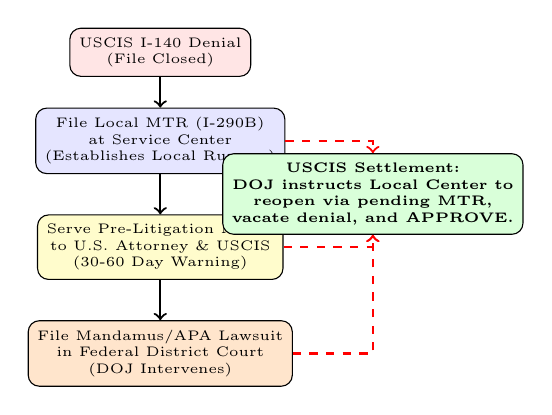
\begin{tikzpicture}[scale=0.45, every node/.style={draw, rounded corners, align=center, font=\tiny}]
				\node (denial) at (0,0) [fill=red!10] {USCIS I-140 Denial\\(File Closed)};
				\node (mtr) at (0,-2.5) [fill=blue!10] {File Local MTR (I-290B)\\at Service Center\\(Establishes Local Runway)};
				\node (notice) at (0,-5.5) [fill=yellow!20] {Serve Pre-Litigation Notice\\to U.S. Attorney \& USCIS\\(30-60 Day Warning)};
				\node (lawsuit) at (0,-8.5) [fill=orange!20] {File Mandamus/APA Lawsuit\\in Federal District Court\\(DOJ Intervenes)};
				\node (settle) at (6,-4) [fill=green!15, font=\bfseries\tiny] {USCIS Settlement:\\DOJ instructs Local Center to\\reopen via pending MTR,\\vacate denial, and APPROVE.};
				
				\draw[->, thick] (denial) -- (mtr);
				\draw[->, thick] (mtr) -- (notice);
				\draw[->, thick] (notice) -- (lawsuit);
				\draw[->, dashed, thick, red] (lawsuit) -| (settle);
				\draw[->, dashed, thick, red] (notice) -| (settle);
				\draw[->, dashed, thick, red] (mtr) -| (settle);
			\end{tikzpicture}
		\end{center}
	\end{frame}
	
	% ============================================================
	% SECTION 15: DECISION MATRIX & ERROR AVOIDANCE (ORIGINAL)
	% ============================================================
	
	\begin{frame}{Decision Matrix: Selecting Your Path (Part 1)}
		\scriptsize
		\begin{block}{Remediation Framework Based on Evidentiary Posture}
			\centering
			\begin{tabular}{|p{4cm}|p{6.5cm}|}
				\hline
				\textbf{Evidentiary Posture} & \textbf{Prescribed Action Path} \\
				\hline
				New expert letters or filing-date metrics are available. & File a local \textbf{Motion to Reopen (MTR)} immediately to establish your settlement baseline. \\
				\hline
				Clear legal misapplication on the existing record with no new facts. & File a joint \textbf{MTR/MTC} to hook both legal errors and new clarifying evidence. \\
				\hline
			\end{tabular}
		\end{block}
	\end{frame}
	
	\begin{frame}{Decision Matrix: Selecting Your Path (Part 2)}
		\scriptsize
		\begin{block}{Remediation Framework Based on Timeline Posture}
			\centering
			\begin{tabular}{|p{4cm}|p{6.5cm}|}
				\hline
				\textbf{Evidentiary Posture} & \textbf{Prescribed Action Path} \\
				\hline
				Local center refuses to rule or stalls the pending MTR for 6+ months. & Issue a formal \textbf{Pre-Litigation Notice}, followed immediately by a federal \textbf{Writ of Mandamus}. \\
				\hline
				Considering an AAO Appeal out of standard reflex. & \textbf{Avoid entirely.} The AAO has no out-of-court settlement authority and completely kills your local leverage. \\
				\hline
			\end{tabular}
		\end{block}
	\end{frame}
	
	\begin{frame}{Decision Matrix: Selecting Your Path (Part 3)}
		\scriptsize
		\begin{block}{Remediation Framework Based on Denial Type}
			\centering
			\begin{tabular}{|p{4cm}|p{6.5cm}|}
				\hline
				\textbf{Denial Type} & \textbf{Prescribed Action Path} \\
				\hline
				Denial based on factual misunderstanding of your evidence. & \textbf{MTR with clarifying evidence.} Show the officer misread or missed key documents. \\
				\hline
				Denial based on legal error (wrong standard, misapplied precedent). & \textbf{MTC focusing on legal argument.} Cite \textit{Dhanasar}, Policy Manual, regulations. \\
				\hline
				Denial based on lack of evidence that you can now supply. & \textbf{Refile} (not appeal). MTR cannot introduce entirely new categories of evidence. \\
				\hline
				Denial that is clearly wrong on both facts and law. & \textbf{Combined MTR/MTC + Pre-Litigation Notice.} Apply maximum pressure. \\
				\hline
			\end{tabular}
		\end{block}
	\end{frame}
	
	\begin{frame}{Common Mistakes That Destroy Cases}
		\scriptsize
		\begin{block}{Fatal Post-Denial Mistakes to Avoid}
			\begin{enumerate}
				\item \textbf{Filing an AAO Appeal out of reflex:} This locks your case file in an appellate queue for months where local settlement is impossible.
				\item \textbf{Filing an MTC alone when you need to add new letters:} Because an MTC strictly forbids new facts, adding evidence causes an automatic, unappealable dismissal.
				\item \textbf{Filing a federal lawsuit without an active local motion:} If you don't have a pending MTR at the local service center, the agency has no fast administrative mechanism to easily reopen and settle your case out of court.
			\end{enumerate}
		\end{block}
	\end{frame}
	
	\begin{frame}{Additional Common Mistakes to Avoid}
		\scriptsize
		\begin{block}{More Fatal Errors}
			\begin{enumerate}
				\item \textbf{Missing the 30-day deadline:} No extensions. If you miss it, your only option is to refile a new I-140.
				\item \textbf{Sending your MTR to the wrong address:} Different service centers handle different case types. Check USCIS website before mailing.
				\item \textbf{Using the wrong fee amount:} USCIS fees change periodically. Check the G-1055 fee schedule on the day you mail.
				\item \textbf{Forgetting to sign Form I-290B:} Unsigned forms are rejected immediately, and you may miss the deadline before resubmitting.
				\item \textbf{Not including proof of service:} You must show you served copies on all relevant government offices.
				\item \textbf{Filing without a legal brief:} Form I-290B alone is insufficient. You must attach a detailed legal argument.
				\item \textbf{Using emotional language:} Stick to facts, law, and evidence. Emotional appeals are ignored.
			\end{enumerate}
		\end{block}
	\end{frame}
	
	% ============================================================
	% SECTION 16: ADVANCED MODULES (ORIGINAL)
	% ============================================================
	
	\begin{frame}{Advanced Field Execution: Overcoming Prong 1 Deficiencies}
		\scriptsize
		\begin{block}{Systemic Errors in Adjudicating National Importance}
			When an officer issues a denial under Prong 1, they frequently confuse the commercial scale of an enterprise with the national importance of the underlying endeavor. To counter this effectively:
			\begin{itemize}
				\item \textbf{Isolate the Endeavor:} Clearly decouple your personal active research or framework implementation from generic employer activities.
				\item \textbf{Establish Broad Industry Repercussions:} Leverage expert opinion declarations to prove that your modeling methodologies are reproducible and offer systemic benefits to financial infrastructures nationwide.
				\item \textbf{Deconstruct Scale Arguments:} Cite \textit{Matter of Dhanasar} directly to highlight that an endeavor need not exhibit geographical ubiquity to have structural national impact.
			\end{itemize}
		\end{block}
	\end{frame}
	
	\begin{frame}{Advanced Field Execution: Overcoming Prong 2 Deficiencies}
		\scriptsize
		\begin{block}{Defending the Petitioner's Capacity to Execute}
			Prong 2 denials typically manifest when an adjudicator asserts that the proposed endeavor lacks immediate operational backing, venture capital injection, or commercial proof of concept. Use these elements in your local response file:
			\begin{itemize}
				\item \textbf{Academic \& Professional Foundations:} Formally introduce detailed tracking portfolios of your doctoral achievements and professional licensing credentials.
				\item \textbf{Prospective Standing:} Argue that demanding finalized market adoption at this stage transforms a forward-looking capacity test into an extra-legal benchmark.
				\item \textbf{Technical Blueprints:} Embed exact historical configuration logs or software deployment outlines executed prior to your filing priority milestone to show active capacity.
			\end{itemize}
		\end{block}
	\end{frame}
	
	\begin{frame}{Advanced Field Execution: Navigating Prong 3 Balancing Metrics}
		\scriptsize
		\begin{block}{Deconstructing the Core Balancing Test}
			The final assessment prong requires demonstrating that waiving a job offer and labor certification is fundamentally advantageous to the economic and structural security interests of the United States. Ensure your brief handles these metrics:
			\begin{itemize}
				\item \textbf{The Certification Conundrum:} Argue that standard labor certifications are mechanically incapable of evaluating specialized analytical intellectual property or algorithmic risk architectures.
				\item \textbf{National Urgency Profiles:} Document the structural relevance of your endeavor to immediate safety, risk management, or regulatory enforcement dockets.
				\item \textbf{Preponderance Safeguards:} Reiterate that under \textit{Matter of Chawathe}, your burden is merely to show that the benefit of a waiver outweighs adherence to standard job-testing protocols.
			\end{itemize}
		\end{block}
	\end{frame}
	
	% ============================================================
	% SECTION 17: CASE STUDY DEEP DIVES (ORIGINAL)
	% ============================================================
	
	\begin{frame}{Case Study Deep Dive: Overturning Adverse Analytics Adjudications}
		\scriptsize
		\begin{block}{The Problem Profile}
			A quantitative researcher focusing on multi-horizon risk analysis within system clearings received an absolute denial from the Texas Service Center. The adjudicator determined that because the work was focused on proprietary institutional clearings, it failed to extend its benefit broadly to the national interest.
		\end{block}
		\begin{block}{The Triage Execution}
			Instead of executing an appeal to the AAO, the applicant initiated a combined Form I-290B Motion to Reopen and Reconsider alongside an immediate digital FOIA petition. This sequence preserved local jurisdiction while forcing the retrieval of internal processing records.
		\end{block}
	\end{frame}
	
	\begin{frame}{Case Study Deep Dive: Resolution Mechanics}
		\scriptsize
		\begin{block}{The Strategic Pivot Sequence}
			The applicant attached three new expert declarations from industry leaders confirming that the system was operational prior to filing, thereby correcting the factual record without running afoul of the \textit{Matter of Katigbak} rule. Concurrently, a formal Pre-Litigation Notice was delivered directly to the local U.S. Attorney's Office.
		\end{block}
		\begin{block}{The Adjudicative Settlement}
			Faced with a highly visible Administrative Procedure Act complaint detailing systemic boilerplate cut-and-paste text in the denial, the Department of Justice attorney directed the service center management to pull the pending local motion, vacate the denial, and enter an absolute approval.
		\end{block}
	\end{frame}
	
	\begin{frame}{Case Study 2: Overcoming a Prong 2 "Well-Positioned" Denial}
		\scriptsize
		\begin{block}{The Problem Profile}
			An independent researcher with a PhD and multiple publications was denied EB2-NIW because USCIS found she was not "well-positioned" to advance her proposed endeavor. The officer noted the absence of a university affiliation or corporate backing.
		\end{block}
		\begin{block}{The Triage Execution}
			The applicant filed an MTR attaching: (1) a detailed 5-year research roadmap with milestones; (2) letters from three senior researchers confirming her methodology was sound; (3) documentation of her prior research output (publications, citations, peer reviews). She argued that \textit{Dhanasar} does not require institutional affiliation.
		\end{block}
		\begin{block}{The Result}
			USCIS reopened and approved. The officer noted that the detailed roadmap and expert letters provided sufficient evidence of capacity to execute.
		\end{block}
	\end{frame}
	
	\begin{frame}{Case Study 3: Using FOIA to Win an MTC}
		\scriptsize
		\begin{block}{The Problem Profile}
			Applicant received a denial that appeared to use boilerplate language. He suspected the officer had not actually read his expert letters.
		\end{block}
		\begin{block}{The FOIA Revelation}
			The FOIA response revealed that the officer's worksheet had no mention of the expert letters. The denial was written by a supervisor using a template.
		\end{block}
		\begin{block}{The MTC Strategy}
			The applicant filed an MTC arguing that the agency had failed to consider highly probative evidence, as demonstrated by the FOIA records. The MTC attached the FOIA response as Exhibit A.
		\end{block}
		\begin{block}{The Result}
			USCIS reopened and approved. The officer could not defend a denial that ignored key evidence.
		\end{block}
	\end{frame}
	
	% ============================================================
	% SECTION 18: PROCEDURAL TIMELINE & LOGISTICAL ENGINEERING (ORIGINAL)
	% ============================================================
	
	\begin{frame}{The 30-Day Operational Tracking Matrix}
		\scriptsize
		\begin{block}{Day-by-Day Post-Denial Recovery Action Items}
			\centering
			\begin{tabular}{|p{2cm}|p{6cm}|p{3cm}|}
				\hline
				\textbf{Timeline Phase} & \textbf{Operational Action Profile} & \textbf{Safeguard Rule} \\
				\hline
				Day 1 & Retrieve absolute denial notice from tracking portal. & Calculate exact deadline dates. \\
				\hline
				Day 2--5 & Launch digital FOIA tracking strings via FIRST. & Target internal worksheets. \\
				\hline
				Day 5--12 & Solicit clarifying expert evaluation letters. & Match historical priority dates. \\
				\hline
				Day 15--20 & Author primary Form I-290B cover brief strings. & Cross-reference exhibit codes. \\
				\hline
				Day 25 & Secure formal tracking delivery at local lockbox. & Archive courier signature cards. \\
				\hline
				Day 30 & Serve Pre-Litigation Notice to the U.S. Attorney. & Execute via certified postal mail. \\
				\hline
			\end{tabular}
		\end{block}
	\end{frame}
	
	\begin{frame}{Logistical Intake Engineering: Eliminating Technical Rejections}
		\scriptsize
		\begin{block}{Preventing Administrative Rejections at Mailroom Checkpoints}
			A significant portion of administrative motions fail to clear the baseline mailroom screening due to clerical entry mistakes. Protect your file from premature rejection:
			\begin{itemize}
				\item \textbf{Signature Verification Protocols:} Ensure that Form I-290B features wet or legally authorized digital signatures. Photocopied signatures frequently trigger an immediate rejection.
				\item \textbf{Fee Calculation Guardrails:} Double-check active G-1055 schedule guidelines on the exact morning of shipping. Using outdated fee benchmarks will cause your package to be returned, costing you your 30-day window.
				\item \textbf{Address Line Audits:} Match the physical address of the lockbox precisely with your chosen courier service rules, distinguishing carefully between USPS and express shipping drop lines.
			\end{itemize}
		\end{block}
	\end{frame}
	
	% ============================================================
	% SECTION 19: UNABRIDGED REGULATORY CODIFICATION (ORIGINAL)
	% ============================================================
	
	\begin{frame}[allowframebreaks]{Statutory Codification: Administrative Blueprints}
		\scriptsize
		\begin{block}{8 C.F.R. § 103.5(a)(2) -- Requirements for Motion to Reopen}
			``A motion to reopen must state the new facts to be proved in the reopened proceeding and be supported by affidavits or other documentary evidence. A motion to reopen an application or petition denied due to abandonment must be filed with evidence that the decision was in error because: The requested evidence was not material to the issue of eligibility; The required initial evidence was submitted with the application or petition, or the request for initial evidence or additional information was complied with during the time allowed...''
		\end{block}
		\framebreak
		\begin{block}{8 C.F.R. § 103.5(a)(3) -- Requirements for Motion to Reconsider}
			``A motion to reconsider must state the reasons for reconsideration and be supported by any pertinent precedent decisions to establish that the decision was based on an incorrect application of law or Service policy. A motion to reconsider a decision on an application or petition must, when filed, also establish that the decision was incorrect based on the evidence of record at the time of the initial decision.''
		\end{block}
		\framebreak
		\begin{block}{5 U.S.C. § 706 -- Scope of Judicial Court Review}
			``To the extent necessary to decision and when presented, the reviewing court shall decide all relevant questions of law, interpret constitutional and statutory provisions, and determine the meaning or applicability of the terms of an agency action. The reviewing court shall—(1) compel agency action unlawfully withheld or unreasonably delayed; and (2) hold unlawful and set aside agency action, findings, and conclusions found to be—(A) arbitrary, capricious, an abuse of discretion, or otherwise not in accordance with law...''
		\end{block}
	\end{frame}
	
	% ============================================================
	% SECTION 20: MASTER EXHIBIT PACKAGING (ORIGINAL)
	% ============================================================
	
	\begin{frame}{Advanced Document Engineering: Structural Exhibit Indexes}
		\scriptsize
		\begin{block}{Assembling an Evidentiary File for Local Adjudicators}
			To ensure your local MTR package survives mailroom screening and is read by an officer, follow this organization scheme:
			\begin{itemize}
				\item \textbf{Primary Indexing:} Feature a clear Exhibit Index immediately following your legal brief. Every document must correspond to a clear, alphabetized tab.
				\item \textbf{Cross-Referencing:} Within your legal brief, cite specific exhibit pages directly (e.g., See Exhibit A-2, Page 14). Never leave an assertion unsupported.
				\item \textbf{Visual Clarity:} Use clear divider sheets between separate exhibits. This mirrors law firm quality and helps the officer navigate the record efficiently.
			\end{itemize}
		\end{block}
	\end{frame}
	
	\begin{frame}{The Complete Pre-Litigation Deployment Verification List}
		\scriptsize
		\begin{block}{Final Quality Verifications Before Mailing Shipment}
			\begin{itemize}
				\item [$\square$] Verify that Form I-290B features a clear checkmark in the local motion selection fields, explicitly avoiding the AAO appeal queue selections.
				\item [$\square$] Audit fee alignments against active G-1055 tables on the afternoon of shipment.
				\item [$\square$] Verify that the primary cover brief, administrative forms, and signature panels feature wet ink executions.
				\item [$\square$] Attach a complete copy of the underlying USCIS absolute denial notice directly to the back of the briefing packet.
				\item [$\square$] Deliver identical certified mail packages to all six named agency and executive addresses.
				\item [$\square$] Retain hard copies of the signature tracking manifest from your courier. This document is your primary evidence of timely filing if a dispute arises.
			\end{itemize}
		\end{block}
	\end{frame}
	
	% ============================================================
	% SECTION 21: QUICK REFERENCE CHARTS (ORIGINAL)
	% ============================================================
	
	\begin{frame}{Quick Reference: Form I-290B Fee Schedule}
		\scriptsize
		\begin{block}{Filing Fees as of 2026}
			\centering
			\begin{tabular}{|p{5cm}|p{3cm}|}
				\hline
				\textbf{Filing Type} & \textbf{Fee} \\
				\hline
				Motion to Reopen (MTR) & \$675 \\
				\hline
				Motion to Reconsider (MTC) & \$675 \\
				\hline
				Combined MTR/MTC & \$675 \\
				\hline
				AAO Appeal & \$675 \\
				\hline
				Fee Waiver Request & Submit Form I-912 \\
				\hline
			\end{tabular}
			\vspace{0.2cm}
			\textcolor{red}{Check USCIS G-1055 before filing - fees change periodically.}
		\end{block}
	\end{frame}
	
	\begin{frame}{Quick Reference: USCIS Service Center Addresses}
		\scriptsize
		\begin{block}{Where to File Form I-290B for I-140 Denials}
			\centering
			\begin{tabular}{|p{4cm}|p{5cm}|}
				\hline
				\textbf{Service Center} & \textbf{Mailing Address} \\
				\hline
				Texas Service Center (TSC) & USCIS Texas Service Center,\\ 6046 N Belt Line Rd, Ste 100,\\ Irving, TX 75038 \\
				\hline
				Nebraska Service Center (NSC) & USCIS Nebraska Service Center,\\ 850 S St,\\ Lincoln, NE 68508 \\
				\hline
				Potomac Service Center (PSC) & USCIS Potomac Service Center,\\ 2200 Potomac Center Dr,\\ Arlington, VA 20598 \\
				\hline
			\end{tabular}
			\vspace{0.2cm}
			\textcolor{blue}{Check your denial notice for which service center issued the decision.}
		\end{block}
	\end{frame}
	
	\begin{frame}{Quick Reference: Key Deadlines Summary}
		\scriptsize
		\begin{block}{Critical Post-Denial Deadlines}
			\centering
			\begin{tabular}{|p{5cm}|p{4cm}|}
				\hline
				\textbf{Action} & \textbf{Deadline} \\
				\hline
				File MTR/MTC/AAO (within U.S.) & 30 days from denial date \\
				\hline
				File MTR/MTC/AAO (outside U.S.) & 33 days from denial date \\
				\hline
				File Mandamus (for delay) & 6+ months after MTR filing \\
				\hline
				File MTC after MTR denial & 30 days from MTR denial \\
				\hline
				Send Pre-Litigation Notice & Before filing APA Complaint \\
				\hline
				File APA Complaint & After notice period expires (30-60 days) \\
				\hline
			\end{tabular}
			\vspace{0.2cm}
			\textcolor{red}{The 30-day deadlines are absolute and cannot be extended.}
		\end{block}
	\end{frame}
	
	\begin{frame}{Quick Reference: Evidence Hierarchy}
		\scriptsize
		\begin{block}{What Evidence Matters Most}
			\centering
			\begin{tabular}{|p{5cm}|p{4cm}|}
				\hline
				\textbf{Evidence Type} & \textbf{Persuasive Weight} \\
				\hline
				.gov citations (Federal Reserve, Science.gov, ERIC) & Highest \\
				\hline
				.edu citations (Harvard, MIT, Stanford) & Very High \\
				\hline
				Expert opinion letters from Ph.D.s & High \\
				\hline
				Peer-reviewed journal publications & High \\
				\hline
				Citation counts (Google Scholar, Scopus) & Medium-High \\
				\hline
				Peer review certificates & Medium \\
				\hline
				Conference presentations & Medium \\
				\hline
				Blog posts or non-peer-reviewed articles & Low \\
				\hline
			\end{tabular}
			\vspace{0.2cm}
			\textcolor{blue}{A single .gov citation can be worth dozens of regular journal citations.}
		\end{block}
	\end{frame}
	
	% ============================================================
	% SECTION 22: FINAL CHECKLISTS AND CLOSING (ORIGINAL)
	% ============================================================
	
	\begin{frame}{Final Checklist Before Filing (MTR/AAO)}
		\scriptsize
		\begin{block}{Pre-Submission Verification}
			\begin{itemize}
				\item [$\square$] Form I-290B fully completed (all fields filled)
				\item [$\square$] Checkbox selected: Motion to Reopen / Reconsider / Appeal (correct one)
				\item [$\square$] Fee amount verified against current G-1055
				\item [$\square$] Payment method correct (check, money order, G-1450)
				\item [$\square$] Signature present (wet ink or authorized digital)
				\item [$\square$] Legal brief attached (not just the form)
				\item [$\square$] Exhibits organized with index
				\item [$\square$] Copy of underlying denial attached
				\item [$\square$] Proof of service attached (if required)
				\item [$\square$] Address verified (correct service center)
				\item [$\square$] Courier tracking obtained
				\item [$\square$] Copy retained for your records
				\item [$\square$] Deadline met (postmark within 30 days)
			\end{itemize}
		\end{block}
	\end{frame}
	
	\begin{frame}{Final Checklist Before Filing (Pre-Litigation Notice)}
		\scriptsize
		\begin{block}{Pre-Submission Verification}
			\begin{itemize}
				\item [$\square$] Recipients identified (DHS Secretary, USCIS Director, U.S. Attorney)
				\item [$\square$] Full address list verified
				\item [$\square$] Notice letter drafted and signed
				\item [$\square$] Draft complaint attached (Exhibit)
				\item [$\square$] Relevant exhibits attached (denial notices, MTR filings)
				\item [$\square$] Return receipt requested on each package
				\item [$\square$] Copies made for your records
				\item [$\square$] Timeline calculated (30-60 days response window)
				\item [$\square$] Follow-up calendar reminder set
			\end{itemize}
		\end{block}
	\end{frame}
	
	\begin{frame}{Final Checklist Before Filing (APA Complaint)}
		\scriptsize
		\begin{block}{Pre-Submission Verification}
			\begin{itemize}
				\item [$\square$] Administrative remedies exhausted (MTR filed and denied or delayed)
				\item [$\square$] Pre-litigation notice sent (and response period expired)
				\item [$\square$] Complaint drafted with all required sections
				\item [$\square$] Civil cover sheet completed (Form JS-44)
				\item [$\square$] Summons forms prepared for each defendant
				\item [$\square$] Filing fee or fee waiver prepared
				\item [$\square$] Exhibits organized and tabbed
				\item [$\square$] Pro se status indicated (if filing without attorney)
				\item [$\square$] Local district court rules reviewed
				\item [$\square$] ECF registration completed (if filing electronically)
			\end{itemize}
		\end{block}
	\end{frame}
	
	\begin{frame}{The Strategic Takeaways}
		\scriptsize
		\begin{block}{Final Core Paradigms}
			\begin{itemize}
				\item \textbf{Denials are not final.} Most denials contain legal errors that can be challenged.
				\item \textbf{Local MTR keeps your case local.} The service center can reopen if you give them a reason.
				\item \textbf{AAO is a trap.} It offers no settlement authority and low reversal rates.
				\item \textbf{FOIA reveals internal errors.} Use it to see what the officer actually wrote.
				\item \textbf{Pre-litigation notices create leverage.} The government will settle rather than litigate clear errors.
				\item \textbf{Federal court is for legal errors, not new evidence.} Use APA for wrong standards, not for missing documents.
				\item \textbf{Document everything.} Every filing, every receipt, every email.
			\end{itemize}
			\vspace{0.3cm}
			\centering
			\textcolor{blue}{\textbf{Build your local record. Apply federal leverage. Force rapid approvals.}}
		\end{block}
	\end{frame}
	
	\begin{frame}{Closing Remarks}
		\scriptsize
		\begin{block}{Final Words of Encouragement}
			\textbf{Remember:}
			\begin{itemize}
				\item USCIS officers make mistakes. Denials are not always correct.
				\item The system has checks and balances - motions, appeals, and courts.
				\item You are your own best advocate. No one cares more about your case than you.
				\item Document everything. Every filing, every receipt, every conversation.
				\item Act quickly. The 30-day deadline is unforgiving.
				\item FOIA is your friend. Internal notes often reveal errors.
				\item AAO is rarely the answer. Use local MTR + federal leverage instead.
				\item Settlement is possible. The government wants to clear its docket.
			\end{itemize}
			\vspace{0.3cm}
			\textcolor{blue}{This course provides the framework. Your diligence and persistence will determine the outcome.}
			\vspace{0.3cm}
			\textcolor{red}{\textbf{The best time to start your post-denial strategy was yesterday.}}
			\textcolor{red}{\textbf{The second best time is now.}}
		\end{block}
	\end{frame}
	
	\begin{frame}{Thank You}
		\centering
		\vspace{1cm}
		\textcolor{blue}{\Large Your Complete Post-Denial Strategy}
		\vspace{0.5cm}
		\begin{itemize}
			\item Act within 30 days
			\item File FOIA immediately
			\item File MTR with new facts (not just disagreement)
			\item If MTR delayed 6+ months → Mandamus
			\item After MTR denied → File MTC (30 days)
			\item After MTC denied → Pre-Litigation Notice
			\item File APA Complaint if no settlement
		\end{itemize}
		\vspace{0.5cm}
		\textcolor{blue}{\Large Good luck with your appeal or lawsuit!}
		\vspace{0.5cm}
		\textcolor{red}{This presentation is for educational purposes only. Consult a qualified immigration attorney for legal advice specific to your case.}
	\end{frame}
	
\end{document}